\paragraph{虚拟博弈协议（Mechanism-Feedback Fictitious Play）}
我们将 Scenario~B 的一次性同时决策扩展为有限轮虚拟博弈，用于检验模型能否在\emph{不暴露理论答案}的条件下，依靠机制反馈实现策略改进。给定固定的场景实例与结算规则，在每轮 $t=1,\ldots,T$ 执行以下闭环：
\begin{enumerate}
  \item \textbf{信念更新}：基于最近 $w$ 轮历史（默认 $w=10$）计算经验频率信念，即对每个用户 $j$ 估计其分享概率 $\hat{p}^{(t)}_j$。
  \item \textbf{同步决策}：所有用户代理在同一轮并行输出二元动作 $a_i^{(t)}\in\{0,1\}$，且当轮不可见他人动作。
  \item \textbf{机制结算}：环境按真实机制计算泄露、补偿、利润与社会福利，并记录轮次级轨迹。
  \item \textbf{结构化反馈}：向下一轮提供可观测统计（历史参与结构与收益后果），但不提供理论均衡集合本身。
\end{enumerate}
收敛判据采用“\textbf{3 轮稳定}”：若最近 3 轮完整行动剖面一致，则提前停止；否则最多运行 $T=50$ 轮。过程评估同时记录每轮与理论均衡分享集合的 Jaccard 相似度轨迹 $J^{(t)}$，用于刻画学习速度与稳定性。

\paragraph{可视化读法与图示设置}
图~\ref{fig:fp-gpt5} 与图~\ref{fig:fp-dsr1} 分别展示 GPT-5 与 deepseek-r1 的虚拟博弈轨迹。每张图上半部分为 $J^{(t)}$ 折线，下半部分为用户-轮次行动热图（蓝色为分享，浅色为不分享），右侧单列标注理论均衡中的分享用户。该表示将“过程收敛”与“结构一致性”放在同一图中，便于比较不同模型的学习动力学。

\begin{figure*}[t]
  \centering
  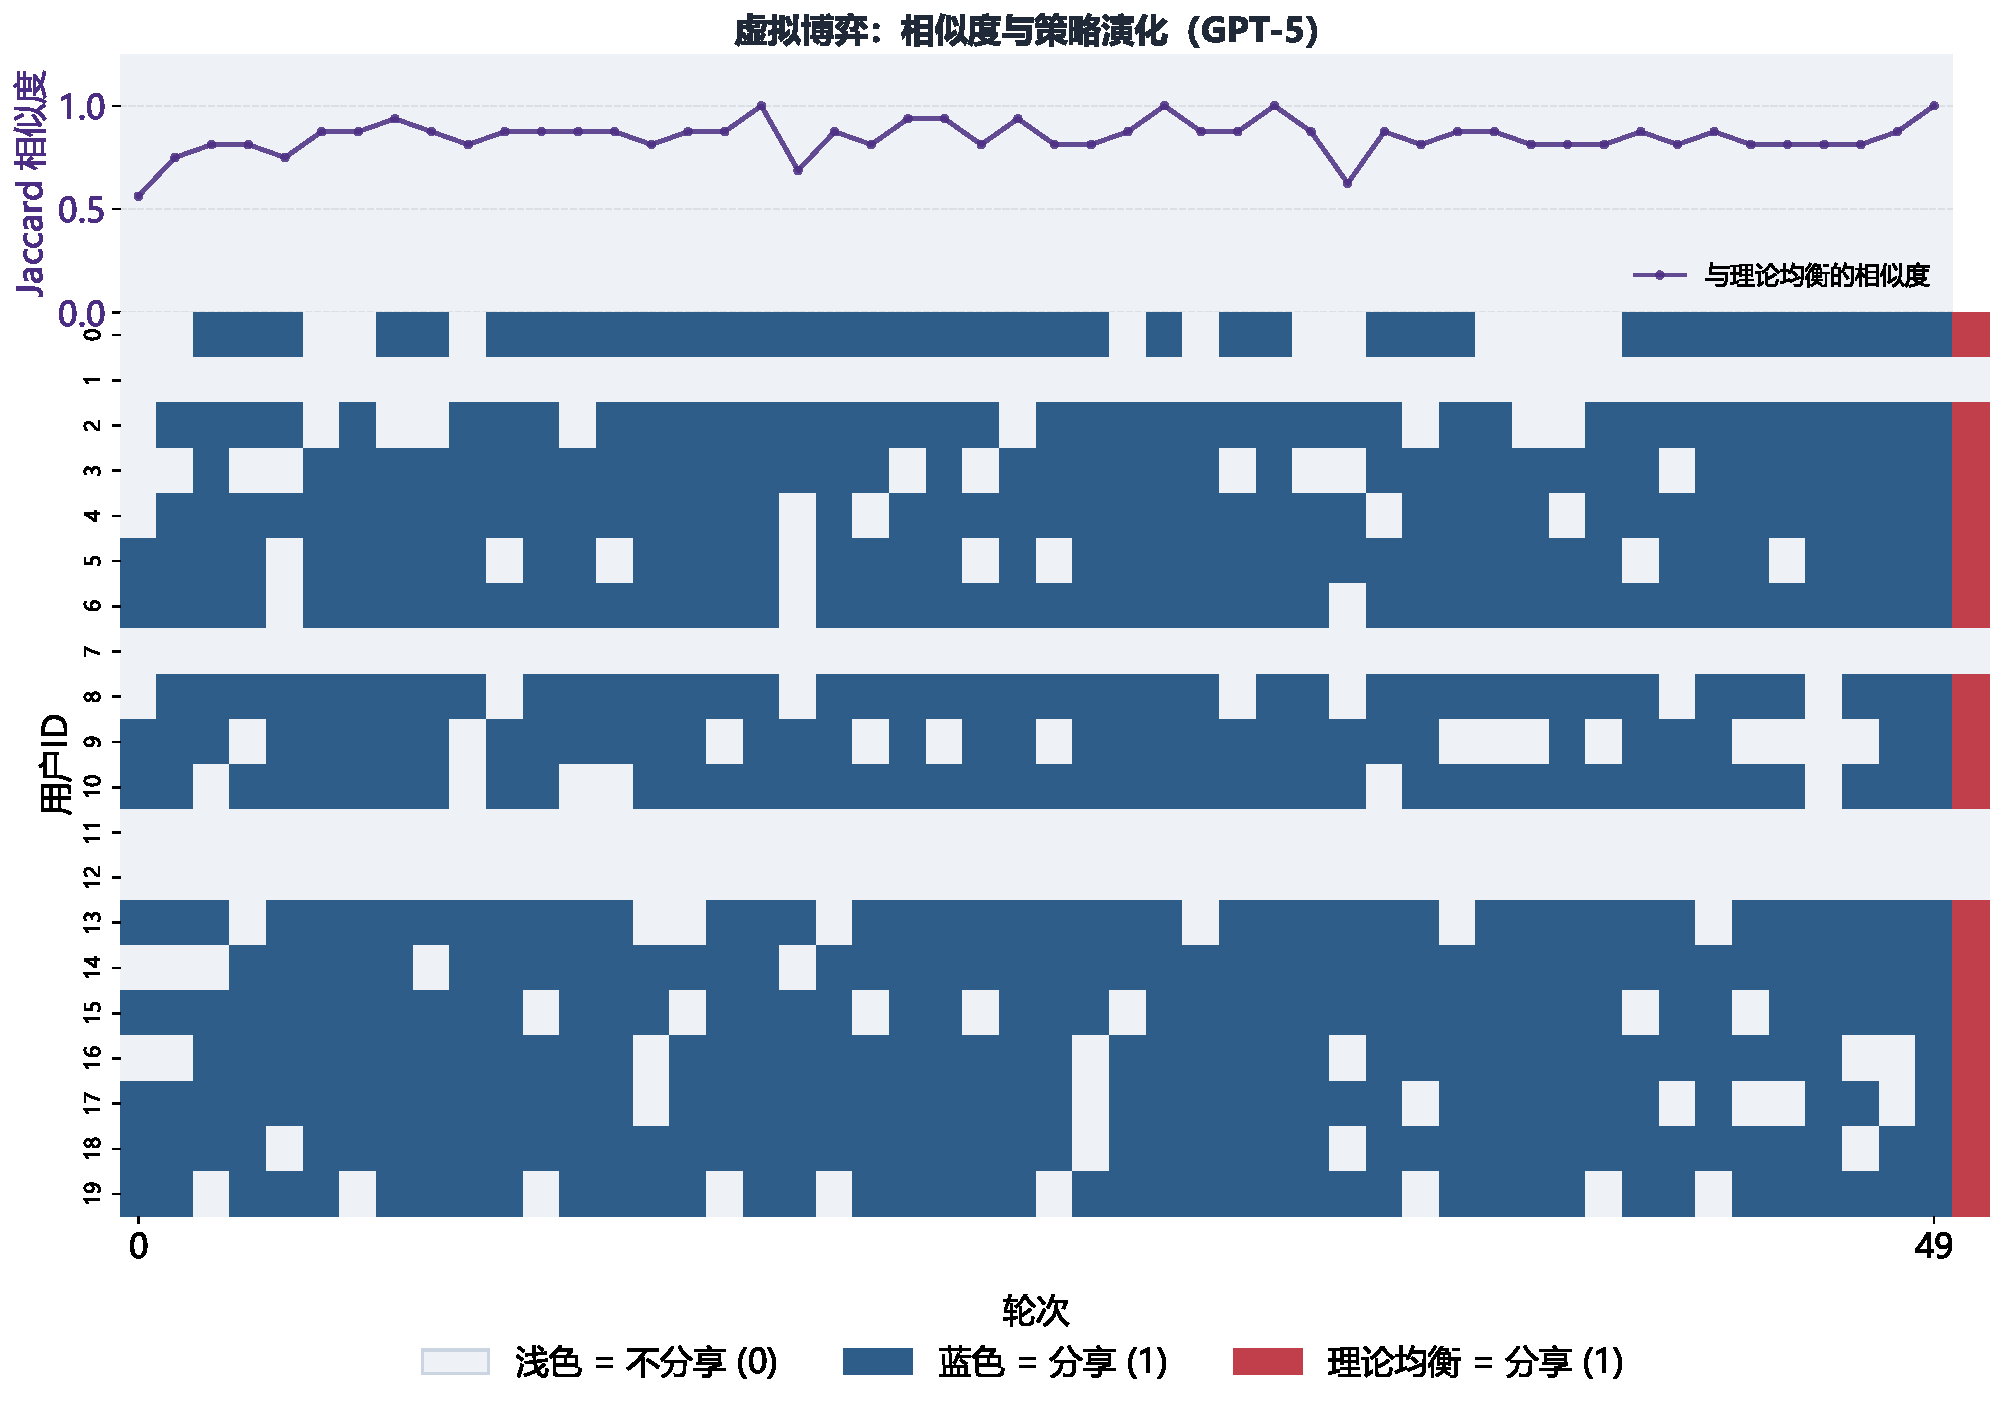
\includegraphics[width=0.94\textwidth]{../evaluation_results/fp_gpt-5/eval_20260204_011138_similarity_heatmap.pdf}
  \caption{Fictitious-play trajectory of \textbf{GPT-5} in Scenario~B. The upper panel reports round-wise Jaccard similarity to the theoretical equilibrium set; the lower panel reports user-level action evolution.}
  \label{fig:fp-gpt5}
\end{figure*}

\begin{figure*}[t]
  \centering
  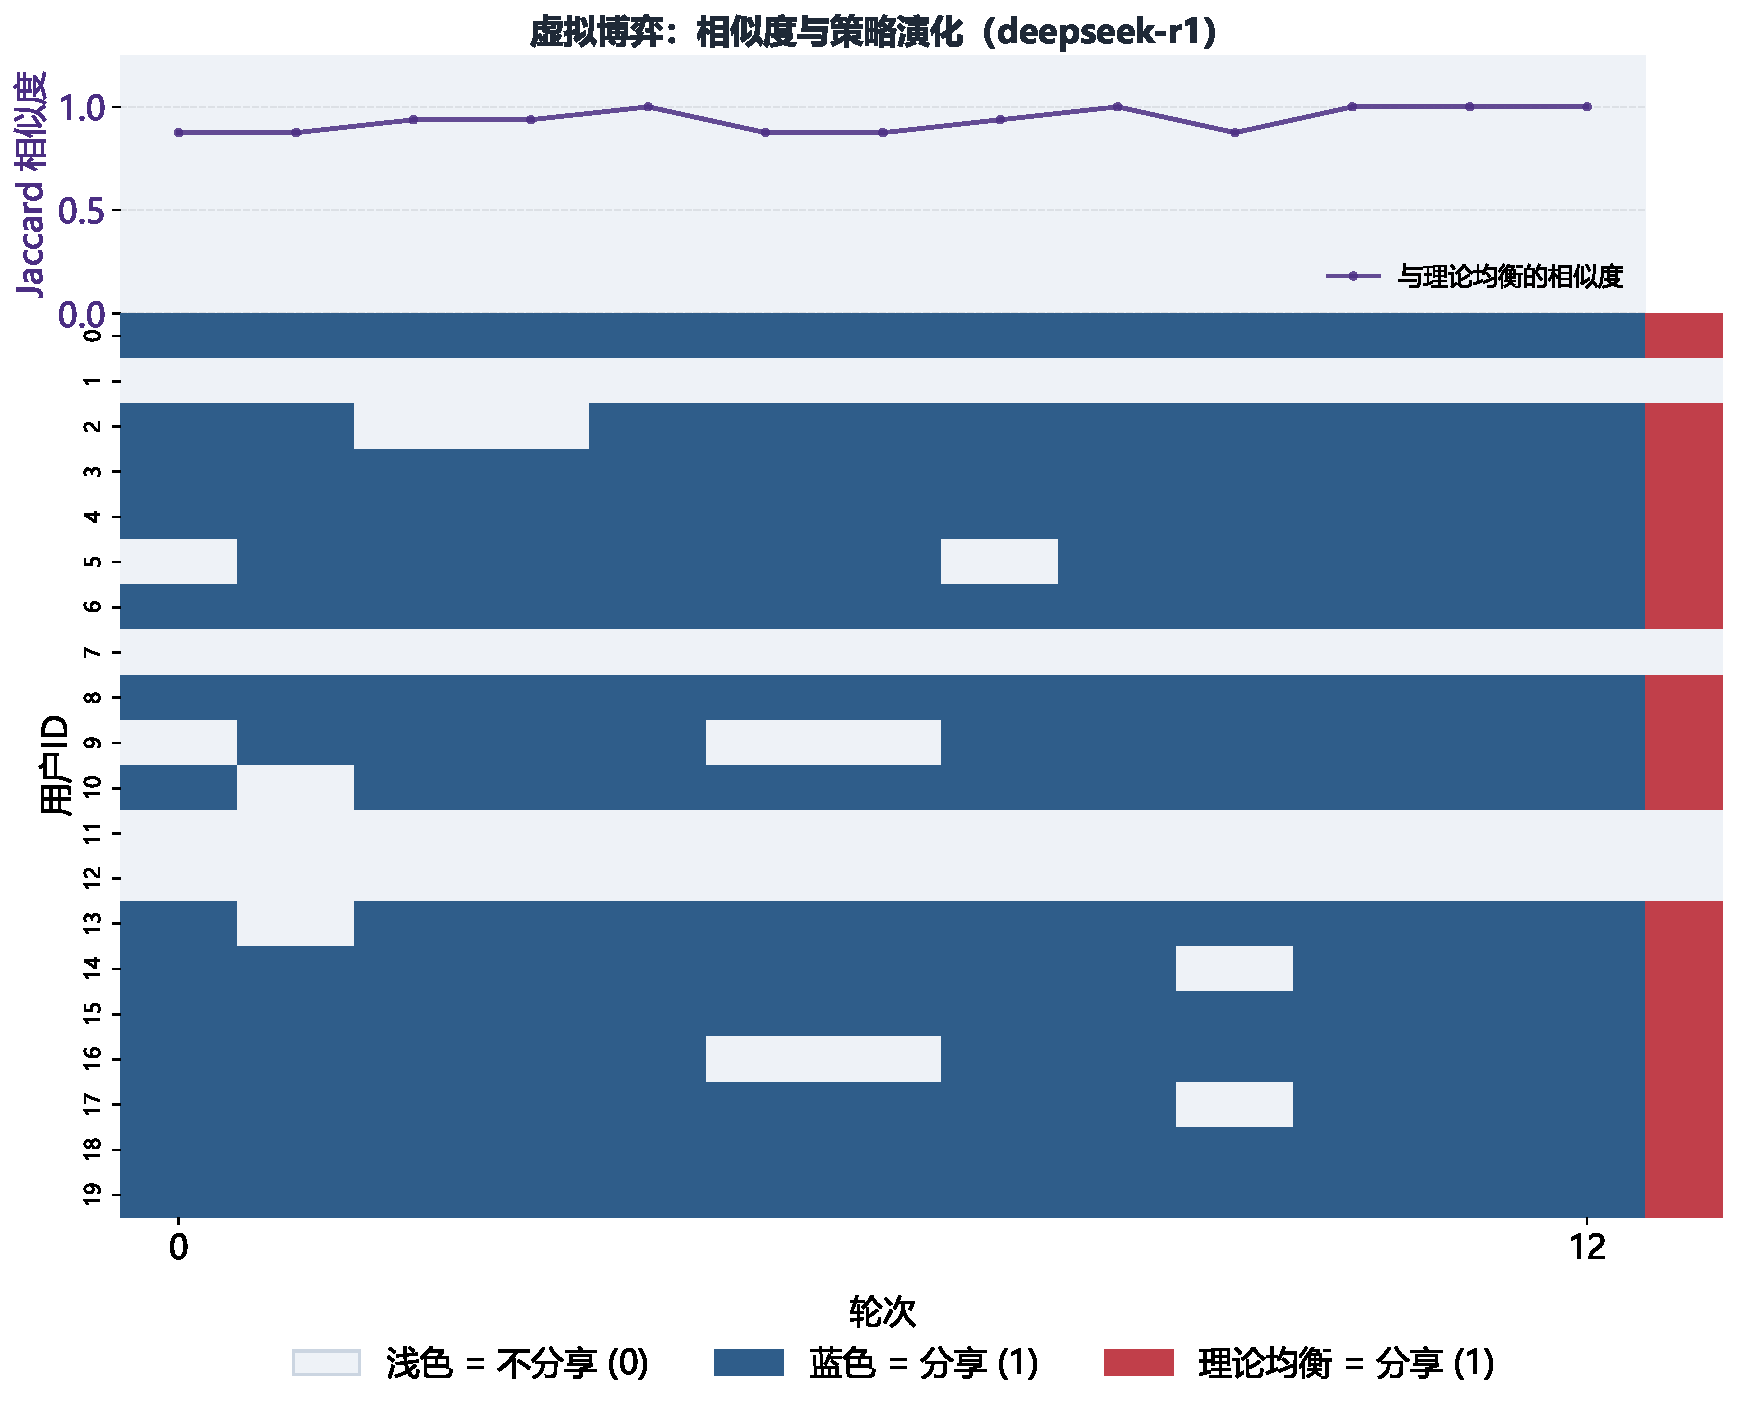
\includegraphics[width=0.94\textwidth]{../evaluation_results/fp_deepseek-r1/eval_20260205_012648_similarity_heatmap.pdf}
  \caption{Fictitious-play trajectory of \textbf{deepseek-r1} in Scenario~B, under the same environment and stopping rule as Figure~\ref{fig:fp-gpt5}.}
  \label{fig:fp-dsr1}
\end{figure*}

\paragraph{结果分析：两类模型均可被机制反馈“拉回”到高一致性区间}
从两条轨迹可以观察到一个共同模式：即使初始轮次并未与理论均衡完全一致，随着机制反馈累积，$J^{(t)}$ 均进入高位并保持稳定。这说明在本任务中，结构化反馈能够将一次性决策中的局部偏差转化为可学习信号，推动策略朝理论结构收敛。

\textbf{GPT-5（图~\ref{fig:fp-gpt5}）}呈现典型的“渐进式修正”路径：相似度先快速上升，再伴随小幅回摆，最后稳定在高一致区间。热图对应地显示，少量用户存在间歇性翻转，但整体行动模式逐步固化。这一形态更接近“持续纠错型”学习器：模型能够利用反馈修正偏差，但需要多轮迭代消化机制信号。

\textbf{deepseek-r1（图~\ref{fig:fp-dsr1}）}则表现为更快的高位聚集与更早停机：在较少轮次内即达到稳定剖面并触发提前终止。热图中多数用户较早锁定动作，仅少数局部单元发生短暂调整。该结果表明 deepseek-r1 对反馈信号的响应更“陡峭”，但其优势主要体现在动态纠偏速度，而非静态一步推理的稳健性。

\paragraph{结论与对主实验的补充意义}
虚拟博弈结果提供了与静态评测互补的证据：
\begin{itemize}
  \item 静态测试回答“模型在单轮是否做对”；
  \item 虚拟博弈回答“模型在机制反馈下是否\emph{学会}做对，以及学得多快、多稳”。
\end{itemize}
因此，Step~3 支持本文核心观点：在外部性机制任务中，终局正确性不足以代表机制理解；过程层面的收敛速度、回摆幅度与稳定区间同样是区分模型能力的重要维度。
